\documentclass[
11pt, % The default document font size, options: 10pt, 11pt, 12pt
% codirector, % Uncomment to add a codirector to the title page
]{charter} 




% El títulos de la memoria, se usa en la carátula y se puede usar el cualquier lugar del documento con el comando \ttitle
\titulo{Desarrollo de un router MIDI configurable} 

% Nombre del posgrado, se usa en la carátula y se puede usar el cualquier lugar del documento con el comando \degreename
\posgrado{Carrera de Especialización en Sistemas Embebidos} 
%\posgrado{Carrera de Especialización en Internet de las Cosas} 
%\posgrado{Carrera de Especialización en Intelegencia Artificial}
%\posgrado{Maestría en Sistemas Embebidos} 
%\posgrado{Maestría en Internet de las cosas}

% Tu nombre, se puede usar el cualquier lugar del documento con el comando \authorname
\autor{Ing. Leandro Martín Soria} 

% El nombre del director y co-director, se puede usar el cualquier lugar del documento con el comando \supname y \cosupname y \pertesupname y \pertecosupname
\director{Dr. Ing. Javier Schandy}
\pertenenciaDirector{FING - UdelaR} 
% FIXME:NO IMPLEMENTADO EL CODIRECTOR ni su pertenencia
\codirector{John Doe} % para que aparezca en la portada se debe descomentar la opción codirector en el documentclass
\pertenenciaCoDirector{FIUBA}

% Nombre del cliente, quien va a aprobar los resultados del proyecto, se puede usar con el comando \clientename y \empclientename
\cliente{Ing. Leandro Martín Soria}
\empresaCliente{Emprendimiento Personal}

% Nombre y pertenencia de los jurados, se pueden usar el cualquier lugar del documento con el comando \jurunoname, \jurdosname y \jurtresname y \perteunoname, \pertedosname y \pertetresname.
\juradoUno{Nombre y Apellido (1)}
\pertenenciaJurUno{pertenencia (1)} 
\juradoDos{Nombre y Apellido (2)}
\pertenenciaJurDos{pertenencia (2)}
\juradoTres{Nombre y Apellido (3)}
\pertenenciaJurTres{pertenencia (3)}
 
\fechaINICIO{22 de agosto de 2023}		%Fecha de inicio de la cursada de GdP \fechaInicioName
\fechaFINALPlan{10 de octubre de 2023} 	%Fecha de final de cursada de GdP
\fechaFINALTrabajo{agosto de 2024}	%Fecha de defensa pública del trabajo final


\begin{document}

\maketitle
\thispagestyle{empty}
\pagebreak


\thispagestyle{empty}
{\setlength{\parskip}{0pt}
\tableofcontents{}
}
\pagebreak


\section*{Registros de cambios}
\label{sec:registro}


\begin{table}[ht]
\label{tab:registro}
\centering
\begin{tabularx}{\linewidth}{@{}|c|X|c|@{}}
\hline
\rowcolor[HTML]{C0C0C0} 
Revisión & \multicolumn{1}{c|}{\cellcolor[HTML]{C0C0C0}Detalles de los cambios realizados} & Fecha      \\ \hline
0      & Creación del documento                                 &\fechaInicioName \\ \hline
1      & Se completa hasta el punto 5 inclusive                 & 3 de septiembre de 2023 \\ \hline
2      & Se completa hasta el punto 9 inclusive                 & 11 de septiembre de 2023 \\ \hline
3      & Se completa hasta el punto 12 inclusive                 & 20 de septiembre de 2023 \\ \hline
%		  Se puede agregar algo más \newline
%		  En distintas líneas \newline
%		  Así                                                    & dd/mm/aaaa \\ \hline
%3      & Se completa hasta el punto 11 inclusive                & dd/mm/aaaa \\ \hline
%4      & Se completa el plan	                                 & dd/mm/aaaa \\ \hline
\end{tabularx}
\end{table}

\pagebreak

\section*{Acta de constitución del proyecto}
\label{sec:acta}

\begin{flushright}
Buenos Aires, \fechaInicioName
\end{flushright}

\vspace{2cm}

Por medio de la presente se acuerda con el \authorname\hspace{1px} que su Trabajo Final de la \degreename\hspace{1px} se titulará ``\ttitle'', consistirá esencialmente en la implementación del prototipo de una interfaz MIDI con opciones de \emph{routing} y filtrado de mensajes (ambos configurables desde una interfaz de usuario), y tendrá un presupuesto preliminar estimado de 674 horas de trabajo y US\$14086,99, con fecha de inicio \fechaInicioName\hspace{1px} y fecha de presentación pública \fechaFinalName.

Se adjunta a esta acta la planificación inicial.

\vfill

% Esta parte se construye sola con la información que hayan cargado en el preámbulo del documento y no debe modificarla
\begin{table}[ht]
\centering
\begin{tabular}{ccc}
\begin{tabular}[c]{@{}c@{}}Dr. Ing. Ariel Lutenberg \\ Director posgrado FIUBA\end{tabular} & \hspace{2cm} & \begin{tabular}[c]{@{}c@{}}\clientename \\ \empclientename \end{tabular} \vspace{2.5cm} \\ 
\multicolumn{3}{c}{\begin{tabular}[c]{@{}c@{}} \supname \\ Director del Trabajo Final\end{tabular}} \vspace{2.5cm} \\
%\begin{tabular}[c]{@{}c@{}}\jurunoname \\ Jurado del Trabajo Final\end{tabular}     &  & \begin{tabular}[c]{@{}c@{}}\jurdosname\\ Jurado del Trabajo Final\end{tabular}  \vspace{2.5cm}  \\
%\multicolumn{3}{c}{\begin{tabular}[c]{@{}c@{}} \jurtresname\\ Jurado del Trabajo Final\end{tabular}} \vspace{.5cm}                                                                     
\end{tabular}
\end{table}

\section{1. Descripción técnica-conceptual del proyecto a realizar}
\label{sec:descripcion}
Es frecuente encontrar en estudios de grabación/producción musical (tanto profesionales como hogareños) una mediana o gran variedad de instrumentos musicales electrónicos, principalmente sintetizadores o unidades de efectos.

Dicho equipamiento suele comunicarse mediante un estándar denominado \textbf{MIDI} (\emph{Musical Instrument Digital Interface}), el cual describe:
\begin{itemize}
	\item Un protocolo de comunicación: cómo se codifican los mensajes MIDI, y a qué velocidad deben transmitirse (de manera serializada).
	\item Una interfaz digital: cómo son los circuitos adaptadores de señales MIDI.
	\item Conectores eléctricos: cómo es la conexión desde un punto de vista eléctrico-mecánico.
\end{itemize}

Cabe destacar que la comunicación MIDI no es solo entre instrumentos, sino que también puede ser entre instrumentos y una computadora personal. Cada uno de los equipos puede ser tanto transmisor como receptor de mensajes. Sin embargo, debe existir un conector para cada dirección, tal como se muestra en la Figura \ref{fig:01-midi-connector}. En ella se observa un conector DIN-5 para enviar datos, otro para recibirlos y otro para la funcionalidad \emph{thru} (explicada más adelante). Si bien el tipo de conector más utilizado es el DIN-5, hoy en día también hay instrumentos capaces de transferir mensajes MIDI vía USB.

\begin{figure}[htpb]
	\centering 
	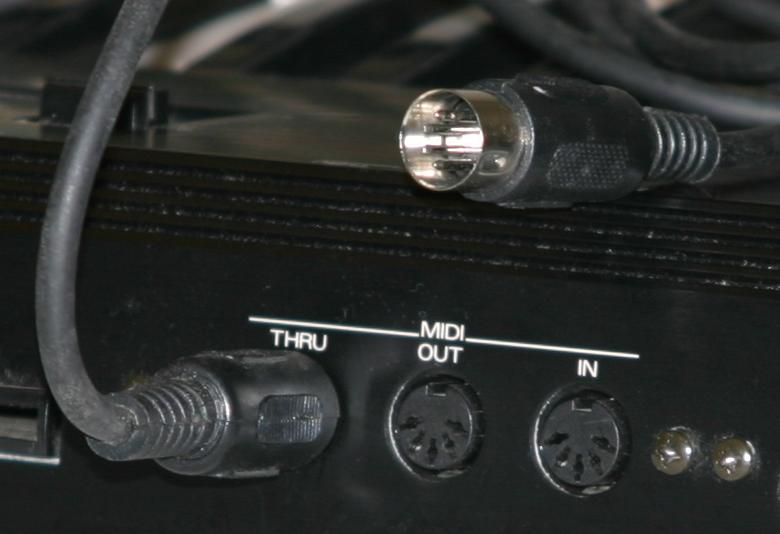
\includegraphics[width=.4\textwidth]{./Figuras/01-midi-connector.jpg}
	\caption{Panel de conectores MIDI de un sintetizador.}
	\label{fig:01-midi-connector}
\end{figure}

Tal como se mencionó aneriormente, algunos equipos poseen un conector adicional denominado \textbf{MIDI THRU}, que retransmite los mensajes recibidos. Esto permite crear topologías denominadas \emph{Daisy Chain}, en las que la salida de un equipo A se conecta a la entrada de un equipo B, y así sucesivamente. Sin embargo, no todos los instrumentos poseen esta característica.

En base a lo mencionado, se puede inferir que se dificulta la interconexión a medida que la cantidad de dispositivos aumenta. La solución a este problema implica el uso de interfaces adicionales que toman una entrada MIDI y la replican en varias salidas. Algunos fabricantes ofrecen equipos con funcionalidades adicionales que permiten realizar un \emph{routeo} de señales más complejo y la capacidad de incluso filtrar mensajes.

El problema es que estos equipos son de fabricación extranjera, y el acceso a los mismos suele ser dificultoso en términos de importación y de costos. Quien redacta este documento se encuentra en esta situación mencionada, y es consciente de otras personas atravesando la misma problemática.

Es por ello que se propone hacer una versión de producción local de menor costo que posea funcionalidades de filtrado y \emph{routeo}, capaz de poder cubrir la demanda local en caso de que se quiera convertir este proyecto personal en un desarrollo comercial.

Para lograr este objetivo se plantea un diagrama en bloques como el de la Figura \ref{fig:diagBloques}, que describe en forma genérica el sistema a desarrollar.

\begin{figure}[htpb]
	\centering 
	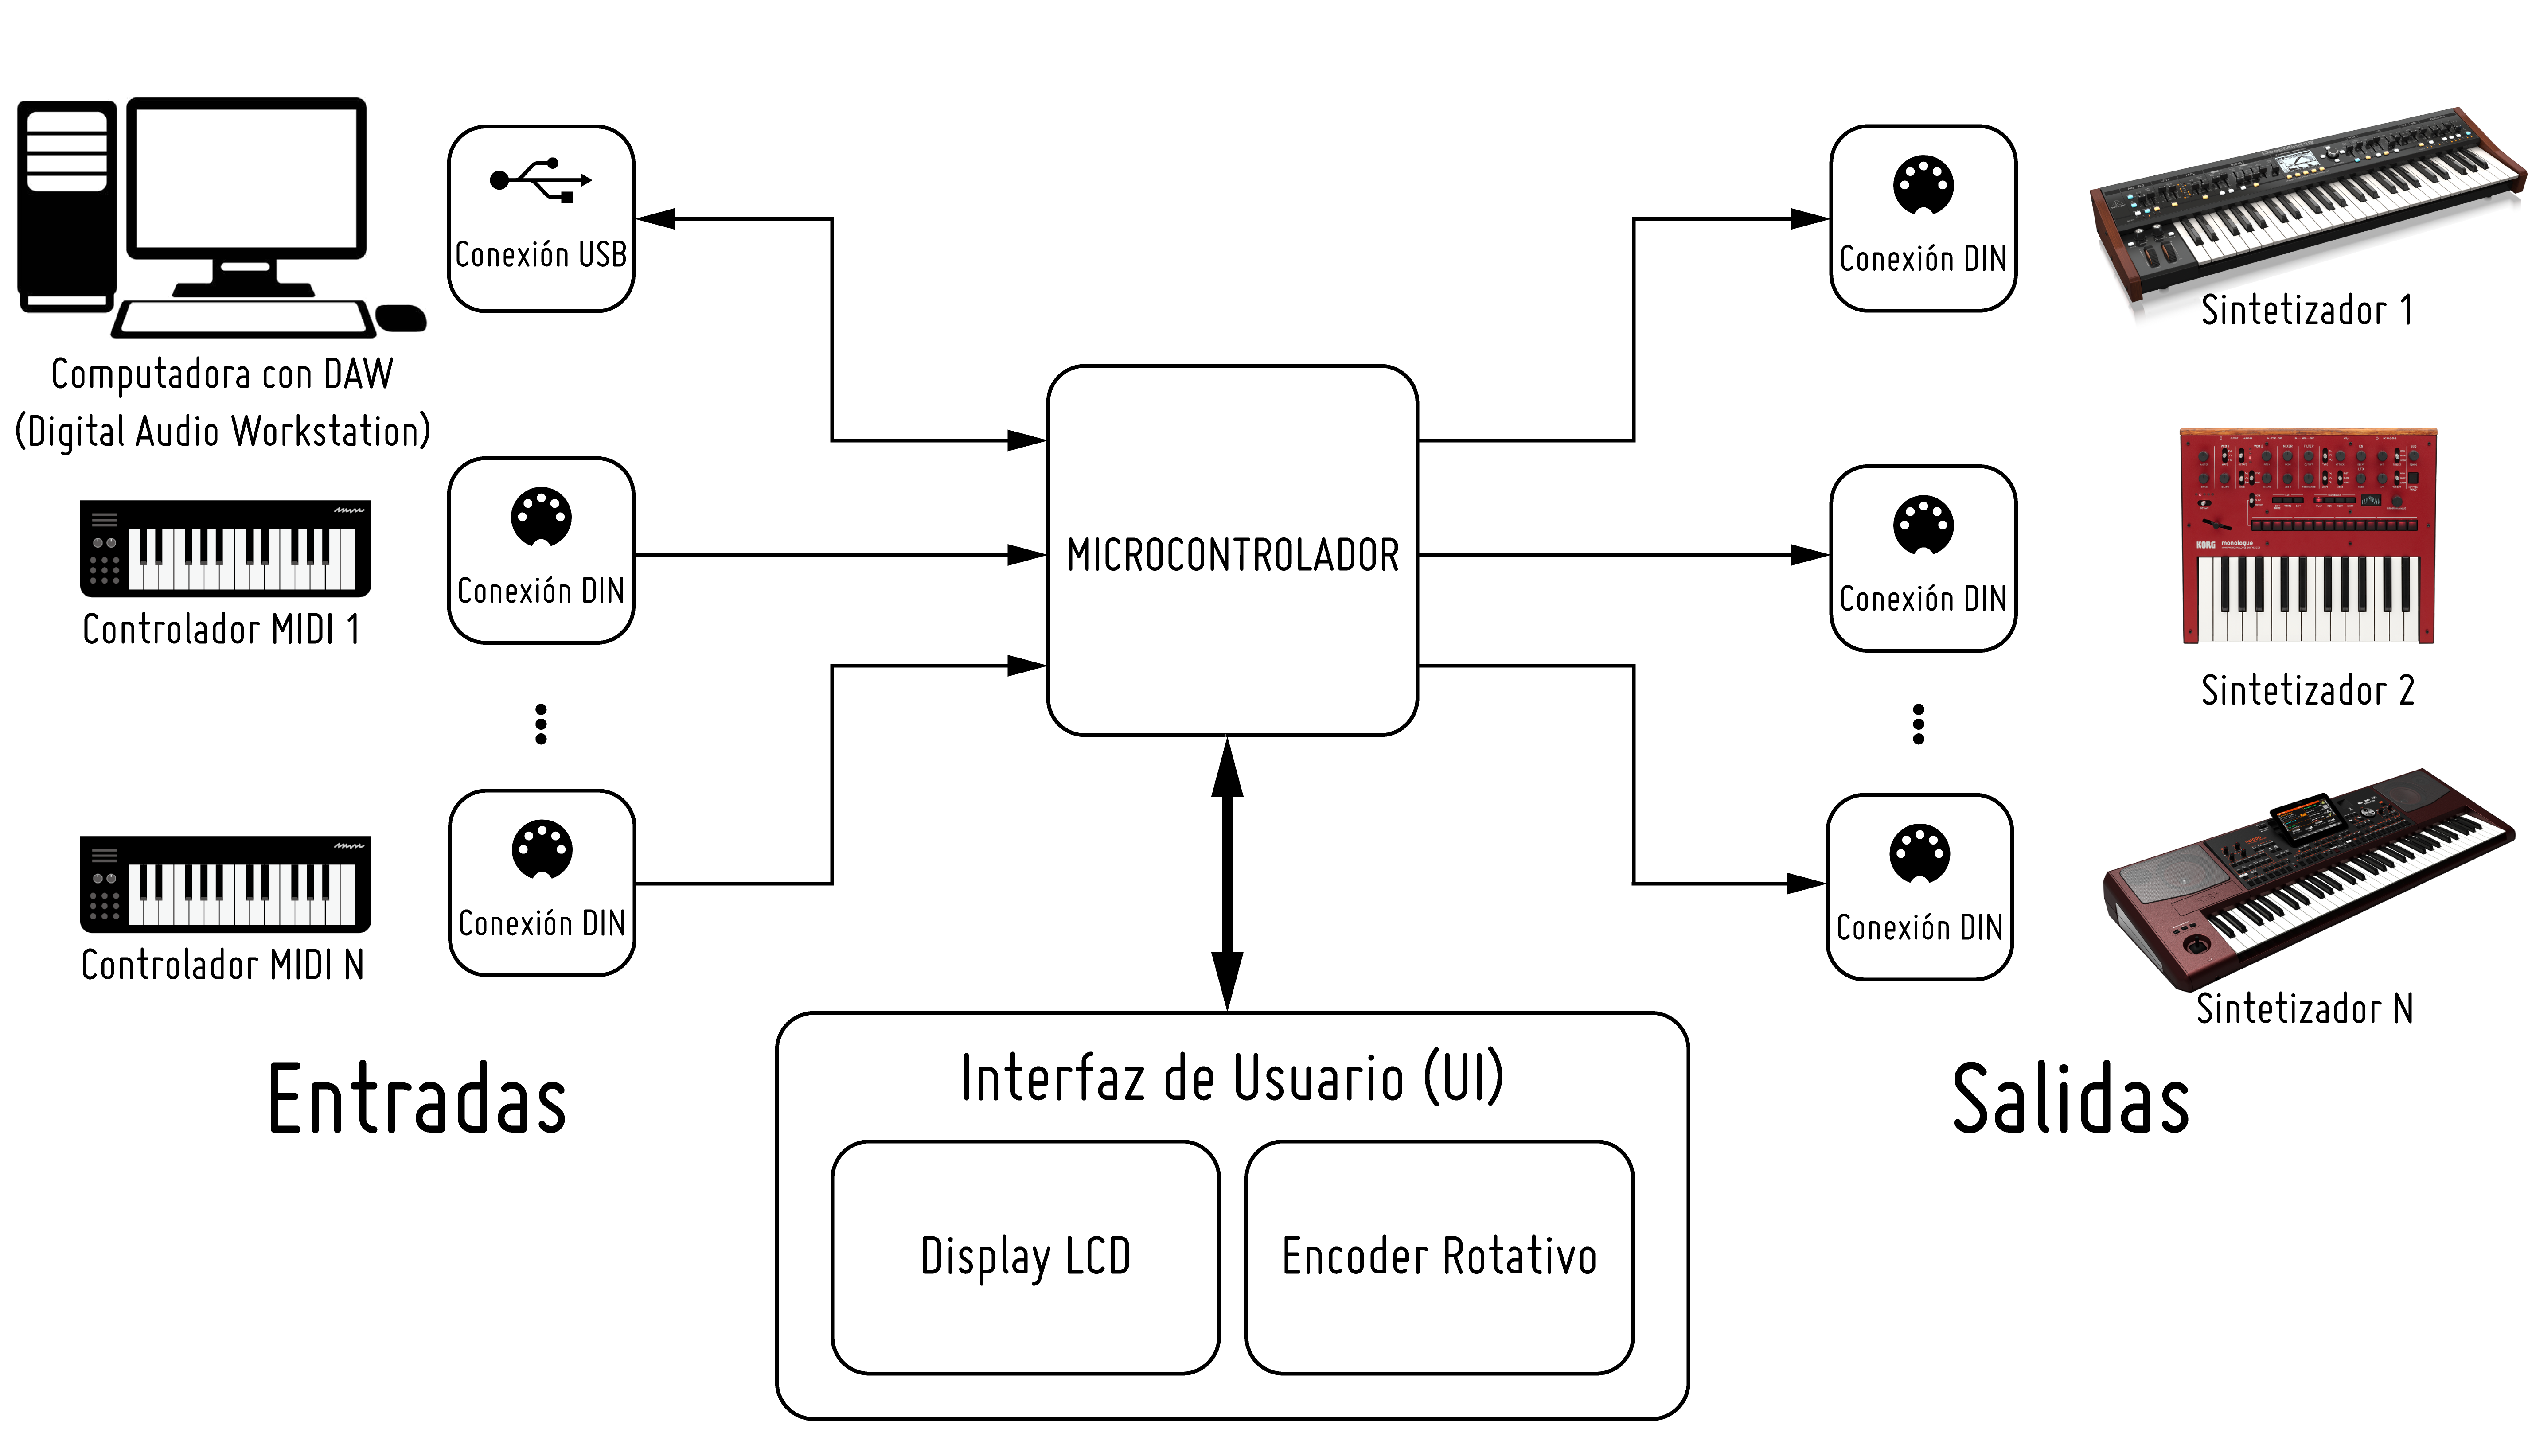
\includegraphics[width=\textwidth]{./Figuras/cese-pf-diagrama.png}
	\caption{Diagrama en bloques del sistema.}
	\label{fig:diagBloques}
\end{figure}

Puede observarse que del lado de la izquierda se muestran las entradas y a la derecha las salidas, ambas utilizando conectores DIN-5. Un microcontrolador será el encargado de procesar el flujo de mensajes.

Esta interfaz (denominada a partir de ahora router) deberá ser configurable por el usuario, tanto en las opciones de routeo como de filtrado de mensajes. La configuración se realizará mediante una interfaz a definir (idealmente un display LCD más un encoder rotativo, aunque se pueden contemplar otras posibilidades como por ejemplo un sitio web embebido).

Pese a que el proyecto es de índole personal, se buscará realizar encuestas sobre la definición de posibles \emph{features} (tanto a nivel hardware como de usabilidad) con la comunidad local (por ejemplo, en foros especializados), de modo de orientar el desarrollo para que eventualmente pueda comercializarse. Este enfoque puede resultar atractivo para potenciales clientes, ya que el desarrollo estaría parcialmente confeccionado en base a requerimientos que el mismo público manifestó.

\newpage

\section{2. Identificación y análisis de los interesados}
\label{sec:interesados}

\begin{table}[ht]
%\caption{Identificación de los interesados}
%\label{tab:interesados}
\begin{tabularx}{\linewidth}{@{}|l|X|X|l|@{}}
\hline
\rowcolor[HTML]{C0C0C0} 
Rol           & Nombre y Apellido & Organización 	& Puesto 	\\ \hline
Cliente       & \clientename      &\empclientename	&   -    	\\ \hline
Responsable   & \authorname       & FIUBA        	& Alumno 	\\ \hline
Colaboradores & Comunidad Local   &      -        	&    -    	\\ \hline
Orientador    & \supname	      & \pertesupname 	& Director Trabajo Final \\ \hline
\end{tabularx}
\end{table}

\begin{itemize}
	\item Colaboradores: dado que va a ser gente de foros de Internet, tener criterio al considerar las opiniones planteadas.
	\item Orientador: Javier Schandy tiene experiencia en RTOS y gestión de proyectos. Aprovechar estas cualidades.
\end{itemize}

\section{3. Propósito del proyecto}
\label{sec:proposito}

El propósito de este proyecto es desarrollar un router MIDI capaz de interconectar los instrumentos musicales que le pertenecen al autor. Por otro lado, se desea que esta experiencia sirva como aprendizaje sobre tecnologías vinculadas a la electrónica musical, y al mismo tiempo permita mostrar el prototipo a la comunidad local de músicos, productores y fabricantes, para evaluar un posterior plan de comercialización.

\section{4. Alcance del proyecto}
\label{sec:alcance}

El presente proyecto incluye la presentación del prototipo de un \emph{router} MIDI funcional. Por lo tanto, abarca los siguientes puntos:

\begin{itemize}
	\item El desarrollo de una biblioteca para manejar mensajes MIDI, portable y que pueda utilizarse en futuros proyectos.
	\item El desarrollo del firmware que correrá en la plataforma embebida.
	\item El diseño del hardware utilizando herramientas CAD.
	\item La fabricación del o de los PCBs (\emph{Printed Circuit Board}, Placa de Circuito Impreso) y el montaje de sus respectivos componentes electrónicos.
	\item El diseño y fabricación del gabinete donde serán montada las placas electrónicas.
\end{itemize}

Por otro lado, el presente proyecto no incluye:
\begin{itemize}
	\item El desarrollo de bibliotecas de manejo de interfaces gráficas, ya que se buscarán alternativas existentes.
	\item El diseño de la fuente de alimentación.
\end{itemize}

\section{5. Supuestos del proyecto}
\label{sec:supuestos}

Para el desarrollo del presente proyecto se supone que:

\begin{itemize}
	\item Se tendrá acceso a distribuidores de componentes electrónicos, con capacidad de compra adecuada para la realización de una cantidad limitada de prototipos (menor a diez unidades).
	\item El responsable del proyecto dispondrá de tres horas diarias para realizarlo a cabo, aumentando la disponibilidad horaria entre diciembre de 2023 y marzo de 2024.
	\item El responsable del proyecto posee los conocimientos para llevar a cabo el proyecto. Sin embargo, en el caso de necesitar ayuda, podrá consultar con docentes de la Carrera de Especialización. 
	\item Se disponen de los instrumentos y herramientas adecuados para realizar el desarrollo electrónico.
	\item Se dispone de un presupuesto inicial de 2000 dólares, pudiendo aumentarse en caso de emergencias e imprevistos.
	\item Se cuenta con el apoyo de voluntarios en la ciudad de Rosario (lugar de residencia del desarrollador) para realizar \emph{tests} de usabilidad.
\end{itemize}

\section{6. Requerimientos}
\label{sec:requerimientos}

\begin{enumerate}
	\item Requerimientos de Entrada-Salida (I/O)
	\begin{enumerate}
		\item El equipo deberá contar con conectores DIN-5.
		\item El equipo deberá tener por lo menos 4 (cuatro) conectores de entrada.
		\item El equipo deberá tener por lo menos 8 (ocho) conectores de salida.
		\item El equipo deberá tener un puerto USB para poder comunicarse con una PC.
		\item Dicho puerto USB deberá poder proveer alimentación al equipo si el consumo total lo permite (opcional).
	\end{enumerate}
	
	\item Requerimientos de la comunicación MIDI
	\begin{enumerate}
		\item El equipo deberá soportar el envío de mensajes MIDI de acuerdo a lo mencionado en el documento \emph{MIDI 1.0 Detailed Specification, Document Version 4.2.1}.
		\item Cada entrada deberá enviar los mensajes recibidos a la(s) salida(s) configuradas por el usuario.
		\item Cada entrada y salida deberá poder detectar los siguientes tipos de mensajes de canal (\emph{Channel Voice Messages}) y filtrarlos de acuerdo a la configuración del usuario:
		\begin{enumerate}
			\item \texttt{Note Off}
			\item \texttt{Note On}
			\item \texttt{Polyphonic Key Pressure}
			\item \texttt{Control Change}
			\item \texttt{Program Change}
			\item \texttt{Channel Pressure}
			\item \texttt{Pitch Bend Change}
		\end{enumerate}
		\item Cada entrada y salida deberá poder detectar los siguientes tipos de mensajes de sistema (\emph{System Common Messages}) y filtrarlos de acuerdo a la configuración del usuario:
		\begin{enumerate}
			\item \texttt{System Exclusive}
			\item \texttt{MIDI Time Code Quarter Frame}
			\item \texttt{Song Position Pointer}
			\item \texttt{Song Select}
			\item \texttt{Tune Request}
			\item \texttt{Timing Clock}
			\item \texttt{Start}
			\item \texttt{Continue}
			\item \texttt{Stop}
			\item \texttt{Active Sensing}
			\item \texttt{Reset}
		\end{enumerate}
		\item En caso de que dos o más entradas quieran enviar mensajes a una misma salida, los mensajes serán enviados por orden de llegada.
		\item Cada salida deberá poder agregar un retardo al envío de los mensajes recibidos, configurable por el usuario (prioridad menor/opcional);
	\end{enumerate}
	
	\item Requerimientos de la comunicación USB
	\begin{enumerate}
		\item El equipo deberá soportar conectividad USB, en modo \emph{device}.
		\item El equipo deberá ser \emph{class-compliant} (es decir, no requerir de drivers adicionales para poder utilizarse desde la PC).
		\item En base a lo anterior, el equipo deberá listarse como un periférico USB-MIDI (\emph{USB-MIDI peripheral}).
		\item Los puertos MIDI de entrada y salida deberán ser accesibles desde la computadora.
		\item Si la configuración del equipo se realizará sobre un sitio web embebido, se deberá poder brindar conectividad ethernet virtual mediante RNDIS (\emph{Remote Network Driver Interface Specification}).
	\end{enumerate}
	
	\item Requerimientos de la interfaz/usabilidad
	\begin{enumerate}
		\item La comunicación Humano-Máquina más elemental se realizará mediante un display LCD (u OLED -a definir-) gráfico y un \emph{encoder} rotativo.
		\item Durante la secuencia de inicialización el display deberá mostrar la versión de firmware que corre en el equipo (opcional).
		\item La configuración de \emph{routeo} y filtrado de mensajes se realizará a través de una aplicación gráfica.
		\item En orden de preferencias, dicha aplicación gráfica será:
		\begin{enumerate}
			\item Una página web embebida en el dispositivo.
			\item Una aplicación de escritorio instalable.
			\item Una aplicación embebida en el equipo, mostrada a través del display.
		\end{enumerate}
	\end{enumerate}
	
	\item Requerimientos de almacenamiento
	\begin{enumerate}
		\item La configuración de \emph{routeo} y filtrado de mensajes se denominará \emph{preset}.
		\item El equipo deberá ser capaz de almacenar al menos 16 (dieciseis) \emph{presets} configurables por el usuario.
		\item La selección de los \emph{presets} deberá ser realizada mediante el \emph{encoder} del panel frontal.
		\item La pantalla LCD deberá mostrar el \emph{preset} activo.
	\end{enumerate}	
	
	\item Requerimientos de testing
	\begin{enumerate}
		\item Se deberá crear una \emph{suite} de tests unitarios para validar la codificación/decodificación de mensajes MIDI.
		\item Se deberá crear una \emph{suite} de tests de integración para validar el \emph{routeo} de mensajes.
		\item Se deberá crear una \emph{suite} de tests de integración para validar el filtrado de mensajes.
		\item Se deberán crear tests que midan la latencia entre la recepción y el envío de mensajes, de modo de poder parametrizarla y minimizarla.
		\item Se deberán realizar tests de usabilidad, de modo de garantizar una experiencia de usuario (UX) fluida y amigable.
	\end{enumerate}
	\item Requerimientos de documentación
	\begin{enumerate}
		\item Se deberán documentar tanto el código de la aplicación como el de las bibliotecas desarrolladas utilizando la herramienta \emph{Doxygen}, y alojar la documentación generada en un repositorio.
		\item Se deberá confeccionar un manual de uso orientado a potenciales usuarios que podrían no contar con conocimiento técnico.
		\item Se deberá confeccionar un documento explicando los fundamentos de la codificación de mensajes MIDI, de modo que sirva como manual de referencia.
		\item Este manual de referencia puede ser un anexo del manual de usuario.
	\end{enumerate}

	\item Requerimientos mecánicos
	\begin{enumerate}
		\item Todo el equipamiento deberá caber en un gabinete tipo \emph{rack} de 1RU (\emph{Rack Unit}, 44,5 mm) con las siguientes dimensiones:
		\begin{enumerate}
			\item Alto: 1U, 1,75 pulgadas (44,5mm)
			\item Ancho: 19 pulgadas (483 mm)
			\item Profundidad: 4,72 pulgadas (120 mm)
		\end{enumerate}
		\item Los siguientes componentes deberán colocarse en el panel posterior del equipo.
		\begin{enumerate}
			\item Conectores DIN de entrada.
			\item Conector USB.
			\item Conector de alimentación (si llegara a ser necesario).
		\end{enumerate}
		\item Los siguientes componentes deberán colocarse en el panel frontal del equipo.
		\begin{enumerate}
			\item Conectores DIN de salida.
			\item LEDs de indicación visual.
			\item Pantalla LCD.
			\item Encoder rotativo.
		\end{enumerate}
	\end{enumerate}
\end{enumerate}

\section{7. Historias de usuarios (\textit{Product backlog})}
\label{sec:backlog}

La siguiente lista de historias de usuarios se confeccionó a partir de plantear la propuesta de proyecto en redes sociales, y posteriormente realizar las siguiente preguntas:
``\emph{¿Qué features les gustaría tener en una interfaz MIDI? ¿Hay alguna recomendación sobre algo en particular?}''

Sobre las preguntas recibidas se aplicó un filtro, dejando las sugerencias más relevantes al proyecto y asignándoles una puntuación de acuerdo al siguiente criterio:
\begin{table}[H]
	\centering
	\resizebox{0.75\textwidth}{!}{%
		\begin{tabular}{|c|c|c|
				>{\columncolor[HTML]{C0C0C0}}c |}
			\hline
			\textbf{\begin{tabular}[c]{@{}c@{}}¿Cuánto se conoce \\ acerca de la tarea?\end{tabular}} & \textbf{¿Dependencias?} & \textbf{\begin{tabular}[c]{@{}c@{}}¿Cuanto tiempo \\ demandará la tarea?\end{tabular}} & \textit{\textbf{Story Points} }                                     \\ \hline
			Todo                                                                                     & Nada                   & Menos de dos horas                                                                    & \textbf{1}                                                 \\
			Casi todo                                                                                & Casi nada              & Medio día                                                                             & \textbf{2}                                                 \\
			Algo                                                                                     & Pocas                  & Hasta dos días                                                                        & \textbf{3}                                                 \\
			Casi nada                                                                                & Algunas                & Algunos días                                                                          & \textbf{5}                                                 \\
			Nada                                                                                     & Muchas                 & Cerca de una semana                                                                   & \cellcolor[HTML]{FFFC9E}{\color[HTML]{F8A102} \textbf{8}}  \\
			Nada                                                                                     & Desconocido            & Más de una semana                                                                     & \cellcolor[HTML]{FFCCC9}{\color[HTML]{FE0000} \textbf{13}} \\ \hline
		\end{tabular}%
	}
\end{table}
\begin{enumerate}
	\item ``\emph{Como usuario, quiero poder programar todas las configuraciones de routeo inteligente desde la PC para facilitar la gestión}''.
	\begin{itemize}
		\item Puntuación: \textbf{5 SP}
	\end{itemize}
	\item ``\emph{Como usuario, quiero que cada entrada y salida MIDI tenga un LED para poder visualizar su actividad}''.
		\begin{itemize}
		\item Puntuación: \textbf{1 SP}
	\end{itemize}
	\item ``\emph{Como usuario, me gustaría poder conservar la configuración aplicada desde el software, de modo que pueda mantenerla persistente cuando lleve el equipo a tocar en vivo y no disponga de una computadora}''.
	\begin{itemize}
		\item Puntuación: \textbf{5 SP}
	\end{itemize}
	
	\item ``\emph{Como usuario, me interesa que el equipo traiga un manual que explique qué es MIDI y cómo se usa de una forma fácil}''.
	\begin{itemize}
		\item Puntuación: \textbf{2 SP}
	\end{itemize}
	\item ``\emph{Como usuario, me gustaría que el equipo sea class compliant y no necesite instalar drivers adicionales}''.
	\begin{itemize}
		\item Puntuación: \textbf{8 SP}
	\end{itemize}
	\item ``\emph{Como usuario, me gustaría que el equipo tenga conectores USB robustos desde un punto de vista mecánico, y que además tenga buena aislación eléctrica}''.
	\begin{itemize}
		\item Puntuación: \textbf{1 SP}
	\end{itemize}
	\item ``\emph{Como usuario, me gustaría que el equipo tenga la opción de retrasar los mensajes MIDI por salida, para poder facilitar la sincronización con equipos que tienen distintas latencias.}''.
	\begin{itemize}
		\item Puntuación: \textbf{3 SP}
	\end{itemize}
\end{enumerate}

\section{8. Entregables principales del proyecto}
\label{sec:entregables}

Una vez finalizado el presente proyecto se entregará:

\begin{itemize}
	\item El prototipo funcional, montado dentro de un gabinete.
	\item El manual de usuario.
	\item El informe final.
\end{itemize}

\section{9. Desglose del trabajo en tareas}
\label{sec:wbs}

\begin{enumerate}
	\item Análisis preliminar (40 h)
	\begin{enumerate}
		\item Estudio sobre la especificación MIDI (8 h)
		\item Investigación sobre \emph{features} pedidas por potenciales clientes (8 h)
		\item Realización del plan del proyecto (24 h)
	\end{enumerate}
	\item Desarrollo de la biblioteca de mensajes MIDI (20 h)
	\begin{enumerate}
		\item Modelado de mensajes (4 h)
		\item Codificación de mensajes (8 h)
		\item Decodificación de mensajes (8 h)
	\end{enumerate}
	
	\item Desarrollo del hardware auxiliar (56 h)
	\begin{enumerate}
		\item Selección de componentes (4 h)
		\item Diseño del esquemático (4 h)
		\item Diseño de los PCBs (4 h)
		\item Fabricación y ensamblado de los PCBs (40 h)
		\item Validación del hardware (4 h)
	\end{enumerate}

	\item Desarrollo del firmware, fase 1: gestión de mensajes MIDI sobre entradas/salidas DIN (88 h)
	\begin{enumerate}
		\item Desarrollo de la arquitectura de la aplicación (8 h)
		\item Recepción y detección de mensajes MIDI (8 h)
		\item Transmisión de mensajes MIDI (8 h)
		\item Extensión de la recepción a más de una entrada (16 h)
		\item Extensión de la transmisión a más de una salida (16 h)
		\item \emph{Routeo} de entradas/salidas (16 h)
		\item Filtrado de mensajes (16 h)
	\end{enumerate}
	
	\item Desarrollo del firmware, fase 2: soporte del display y encoder (24 h)
	\begin{enumerate}
		\item Agregar soporte para el encoder rotativo (8 h)
		\item Agregar bibliotecas para manejo del display (16 h)
	\end{enumerate}
	
	\item Desarrollo del firmware, fase 3: soporte USB (88 h)
	\begin{enumerate}
		\item Agregar soporte USB \emph{device} (8 h)
		\item Agregar soporte para interfaz MIDI (32 h)
		\item Agregar soporte para interfaz RNDIS (32 h)
		\item Integración de la interfaz MIDI con el firmware preexistente (16 h)
	\end{enumerate}
	
	\item Desarrollo de la aplicación (80 h)
	\begin{enumerate}
		\item Bocetado de la interfaz gráfica (8 h)
		\item Modelado de la arquitectura de la aplicación (8 h)
		\item Comunicación aplicación - firmware (16 h)
	\end{enumerate}
	
	\item Desarrollo del firmware, fase 4: integración (32 h)
	\begin{enumerate}
		\item Integración entre configuración de la aplicación con el firmware (8 h)
		\item Almacenamiento de configuraciones en memoria no volátil (8 h)
		\item Agregado de \emph{features} adicionales (16 h)
	\end{enumerate}
	
	\item Testing (72 h)
	\begin{enumerate}
		\item Tests unitarios para codificación/decodificación de mensajes MIDI (8 h)
		\item Tests de \emph{routeo} de mensajes (8 h)
		\item Tests de filtrado de mensajes (8 h)
		\item Tests de integración (8 h)
		\item Tests de usabilidad (8 h)
		\item Corrección de errores (16 h)
	\end{enumerate}
	
	\item Desarrollo del hardware (72 h)
	\begin{enumerate}
		\item Selección de componentes (8 h)
		\item Diseño del esquemático (8 h)
		\item Diseño de los PCBs (8 h)
		\item Fabricación y ensamblado de los PCBs (40 h)
		\item Validación del hardware (8 h)
	\end{enumerate}

	\item Desarrollo del gabinete (58 h)
	\begin{enumerate}
		\item Diseño del gabinete (8 h)
		\item Mecanizado del gabinete (40 h)
		\item Montaje del equipo (2 h)
		\item Validación del montaje (8 h)
	\end{enumerate}
	
	\item Documentación (80 h)
	\begin{enumerate}
		\item Informe de avance (4 h)
		\item Redacción del manual de usuario (24 h)
		\item Redacción de las memorias técnicas (24 h)
		\item Armado de la presentación final (8 h)
	\end{enumerate}
\end{enumerate}

\textbf{Cantidad total de horas: (674 h)}

\newpage

\section{10. Diagrama de Activity On Node}
\label{sec:AoN}

En la Figura \ref{fig:AoN} se muestra el diagrama de \emph{Activity on Node} obtenido del desglose de las tareas de la sección \ref{sec:wbs}, asumiendo la posibilidad de paralelizar las tareas. El camino crítico arrojado es de 384 horas.

\begin{figure}[htpb]
\centering 
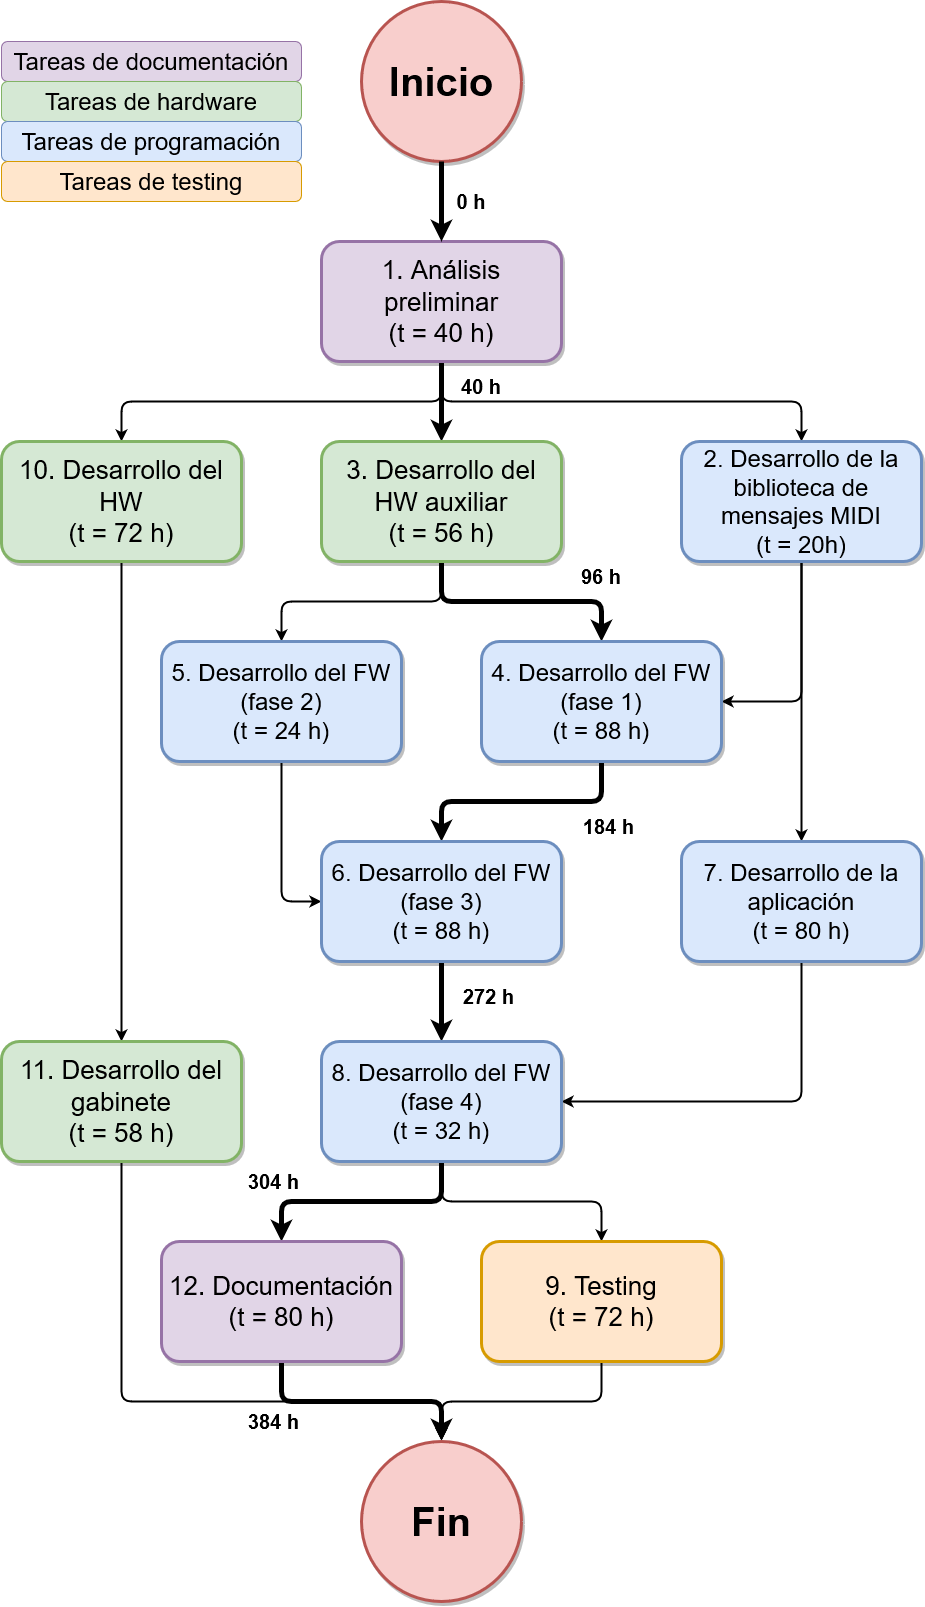
\includegraphics[width=0.66\textwidth]{./Figuras/gdp-aon.png}
\caption{Diagrama de \textit{Activity on Node}.}
\label{fig:AoN}
\end{figure}


\section{11. Diagrama de Gantt}
\label{sec:gantt}

En el Cuadro \ref{tab:gantt-table} se muestra el desglose de tareas de la sección \ref{sec:wbs} tabulado luego de armar el correspondiente diagrama de Gantt. Este diagrama puede consultarse en la Figura \ref{fig:diagGantt}. Para realizar el mismo se asumió que, exceptuando las etapas de manufactura, el único recurso humano es el responsable del proyecto. Por otro lado, se tomó como referencia una jornada laboral de cuatro horas. Además, los días de cierre son los martes y jueves (coincidentes con los días de cursada de la CESE), hasta la finalización del tercer bimestre en diciembre de 2023 (momento de mayor disponibilidad horaria tal como se mencionó entre los supuestos de la sección \ref{sec:supuestos}).
\begin{longtable}[c]{|cllcl|}
	\hline
	\rowcolor[HTML]{C0C0C0} 
	{\color[HTML]{000000} \textbf{WBS}} & \multicolumn{1}{c}{\cellcolor[HTML]{C0C0C0}{\color[HTML]{000000} \textbf{Nombre}}} & \multicolumn{1}{c}{\cellcolor[HTML]{C0C0C0}{\color[HTML]{000000} \textbf{Inicio}}} & {\color[HTML]{000000} \textbf{Duración}} & \multicolumn{1}{c|}{\cellcolor[HTML]{C0C0C0}{\color[HTML]{000000} \textbf{Fin}}} \\ \hline
	\endhead
	%
	\hline
	\endfoot
	%
	\endlastfoot
	%
	\rowcolor[HTML]{ECF4FF} 
	\textbf{1} & \multicolumn{1}{c}{\cellcolor[HTML]{ECF4FF}\textbf{Análisis preliminar}} & \textbf{10/09/23} & \textbf{12 días} & \textbf{16/10/23} \\
	1.1 & Estudio sobre la especificación MIDI & 10/09/23 & 2 días & 11/09/23 \\
	\rowcolor[HTML]{EFEFEF} 
	1.2 & \begin{tabular}[c]{@{}l@{}}Investigación sobre features\\ pedidas por potenciales clientes\end{tabular} & 13/09/23 & 3 días & 15/09/23 \\
	1.3 & Realización del plan del proyecto & 16/09/23 & 6 días & 16/10/23 \\
	\rowcolor[HTML]{ECF4FF} 
	\textbf{2} & \multicolumn{1}{c}{\cellcolor[HTML]{ECF4FF}\textbf{Desarrollo de la biblioteca de mensajes MIDI}} & \textbf{30/10/23} & \textbf{5 días} & \textbf{03/11/23} \\
	2.1 & Modelado de mensajes & 30/10/23 & 1 día & 30/10/23 \\
	\rowcolor[HTML]{EFEFEF} 
	2.2 & Codificación de mensajes & 01/11/23 & 2 días & 03/11/23 \\
	2.3 & Decodificación de mensajes & 01/11/23 & 2 días & 03/11/23 \\
	\rowcolor[HTML]{ECF4FF} 
	\textbf{3} & \multicolumn{1}{c}{\cellcolor[HTML]{ECF4FF}\textbf{Desarrollo del hardware auxiliar}} & \textbf{18/10/23} & \textbf{9 días} & \textbf{29/10/23} \\
	3.1 & Selección de componentes & 18/10/23 & 1 día & 18/10/23 \\
	\rowcolor[HTML]{EFEFEF} 
	3.2 & Diseño de los esquemáticos & 20/10/23 & 1 día & 20/10/23 \\
	3.3 & Diseño de los PCBs & 21/10/23 & 1 día & 21/10/23 \\
	\rowcolor[HTML]{EFEFEF} 
	3.4 & Fabricación y ensamblado de los PCBs & 22/10/23 & 5 días & 28/10/23 \\
	3.5 & Validación del hardware & 29/10/23 & 1 día & 29/10/23 \\
	\rowcolor[HTML]{ECF4FF} 
	\textbf{4} & \multicolumn{1}{c}{\cellcolor[HTML]{ECF4FF}\textbf{Desarrollo del FW (fase 1)}} & \textbf{04/11/23} & \textbf{27 días} & \textbf{03/12/23} \\
	4.1 & Desarrollo de la arquitectura de la aplicación & 04/11/23 & 2 días & 05/11/23 \\
	\rowcolor[HTML]{EFEFEF} 
	4.2 & Recepción y detección de mensajes  MIDI & 06/11/23 & 3 días & 08/11/23 \\
	4.3 & Transmisión de mensajes MIDI & 10/11/23 & 2 días & 11/11/23 \\
	\rowcolor[HTML]{EFEFEF} 
	4.4 & Extensión de la recepción a más de una entrada & 12/11/23 & 6 días & 17/11/23 \\
	4.5 & Extensión de la transmisión a más de una salida & 18/11/23 & 5 días & 22/11/23 \\
	\rowcolor[HTML]{EFEFEF} 
	4.6 & Routeo de entradas/salidas & 24/11/23 & 4 días & 27/11/23 \\
	4.7 & Filtrado de mensajes & 29/11/23 & 5 días & 03/12/23 \\
	\rowcolor[HTML]{ECF4FF} 
	\textbf{5} & \multicolumn{1}{c}{\cellcolor[HTML]{ECF4FF}\textbf{Desarrollo del FW (fase 2)}} & \textbf{04/12/23} & \textbf{7 días} & \textbf{11/12/23} \\
	5.1 & Agregar soporte para el encoder rotativo & 04/12/23 & 3 días & 06/12/23 \\
	\rowcolor[HTML]{EFEFEF} 
	5.2 & Agregar bibliotecas para el manejo del display & 08/12/23 & 4 días & 11/12/23 \\
	\rowcolor[HTML]{ECF4FF} 
	\textbf{6} & \multicolumn{1}{c}{\cellcolor[HTML]{ECF4FF}\textbf{Desarrollo del FW (fase 3)}} & \textbf{12/12/23} & \textbf{27 días} & \textbf{07/01/24} \\
	6.1 & Agregar soporte USB device & 12/12/23 & 2 días & 13/12/23 \\
	\rowcolor[HTML]{EFEFEF} 
	6.2 & Agregar soporte para interfaz MIDI & 14/12/23 & 8 días & 21/12/23 \\
	6.3 & Agregar soporte para interfaz RNDIS & 22/12/23 & 13 días & 03/01/24 \\
	\rowcolor[HTML]{EFEFEF} 
	6.4 & \begin{tabular}[c]{@{}l@{}}Integración de la interfaz MIDI\\ con el FW preexistente\end{tabular} & 04/01/24 & 4 días & 07/01/24 \\
	\rowcolor[HTML]{ECF4FF} 
	\textbf{7} & \multicolumn{1}{c}{\cellcolor[HTML]{ECF4FF}\textbf{Desarrollo de la aplicacióm}} & \textbf{08/01/24} & \textbf{8 días} & \textbf{15/01/24} \\
	7.1 & Bocetado de la interfaz gráfica & 08/01/24 & 2 días & 09/01/24 \\
	\rowcolor[HTML]{EFEFEF} 
	7.2 & Modelado de la arquitectura de la aplicación & 10/01/24 & 2 días & 11/01/24 \\
	7.3 & Comunicación aplicación - firmware & 12/01/24 & 4 días & 15/01/24 \\
	\rowcolor[HTML]{ECF4FF} 
	\textbf{8} & \multicolumn{1}{c}{\cellcolor[HTML]{ECF4FF}\textbf{Desarrollo del FW (fase 4)}} & \textbf{16/01/24} & \textbf{8 días} & \textbf{23/01/24} \\
	8.1 & \begin{tabular}[c]{@{}l@{}}Integración entre configuración \\ de la aplicación con el FW\end{tabular} & 16/01/24 & 2 días & 17/01/24 \\
	\rowcolor[HTML]{EFEFEF} 
	8.2 & \begin{tabular}[c]{@{}l@{}}Almacenamiento de configuraciones\\ en memoria no volátil\end{tabular} & 18/01/24 & 2 días & 19/01/24 \\
	8.3 & Agregado de features adicionales & 20/01/24 & 4 días & 23/01/24 \\
	\rowcolor[HTML]{ECF4FF} 
	\textbf{9} & \multicolumn{1}{c}{\cellcolor[HTML]{ECF4FF}\textbf{Testing}} & \textbf{24/01/24} & \textbf{14 días} & \textbf{06/02/24} \\
	9.1 & \begin{tabular}[c]{@{}l@{}}Tests unitarios para codificación\\ y decodificación de mensajes MIDI\end{tabular} & 24/01/24 & 2 días & 25/01/24 \\
	\rowcolor[HTML]{EFEFEF} 
	9.2 & Tests de routeo de mensajes & 26/01/24 & 2 días & 27/01/24 \\
	9.3 & Tests de filtrado de mensajes & 28/01/24 & 2 días & 29/01/24 \\
	\rowcolor[HTML]{EFEFEF} 
	9.4 & Tests de integración & 30/01/24 & 2 días & 31/01/24 \\
	9.5 & Tests de usabilidad & 01/02/24 & 2 días & 02/02/24 \\
	\rowcolor[HTML]{EFEFEF} 
	9.6 & Corrección de errores & 03/02/24 & 4 días & 06/02/24 \\
	\rowcolor[HTML]{ECF4FF} 
	\textbf{10} & \multicolumn{1}{c}{\cellcolor[HTML]{ECF4FF}\textbf{Desarrollo del hardware}} & \multicolumn{1}{c}{\cellcolor[HTML]{ECF4FF}\textbf{07/02/24}} & \textbf{13 días} & \multicolumn{1}{c|}{\cellcolor[HTML]{ECF4FF}\textbf{19/02/24}} \\
	10.1 & Selección de componentes & 07/02/24 & 2 días & 08/02/24 \\
	\rowcolor[HTML]{EFEFEF} 
	10.2 & Diseño del esquemático & 09/02/24 & 2 días & 10/02/24 \\
	10.3 & Diseño de los PCBs & 11/02/24 & 2 días & 12/02/24 \\
	\rowcolor[HTML]{EFEFEF} 
	10.4 & Fabricación y ensamblado de los PCBs & 13/02/24 & 5 días & 17/02/24 \\
	10.5 & Validación del hardware & 18/02/24 & 2 días & 19/02/24 \\
	\rowcolor[HTML]{ECF4FF} 
	\textbf{11} & \multicolumn{1}{c}{\cellcolor[HTML]{ECF4FF}\textbf{Desarrollo del gabinete}} & \textbf{13/02/24} & \textbf{10 días} & \textbf{22/02/24} \\
	11.1 & Diseño del gabinete & 13/02/24 & 2 días & 14/02/24 \\
	\rowcolor[HTML]{EFEFEF} 
	11.2 & Mecanizado del gabinete & 15/02/24 & 5 días & 19/02/24 \\
	11.3 & Montaje del equipo & 20/02/24 & 1 día & 20/02/24 \\
	\rowcolor[HTML]{EFEFEF} 
	11.4 & Validación del montaje & 21/02/24 & 2 días & 22/02/24 \\
	\rowcolor[HTML]{ECF4FF} 
	{\color[HTML]{000000} \textbf{12}} & \multicolumn{1}{c}{\cellcolor[HTML]{ECF4FF}{\color[HTML]{000000} \textbf{Documentación}}} & {\color[HTML]{000000} \textbf{23/02/24}} & {\color[HTML]{000000} \textbf{}} & {\color[HTML]{000000} \textbf{11/03/24}} \\
	12.1 & Informe de avance &  & 1 día &  \\
	\rowcolor[HTML]{EFEFEF} 
	12.2 & Redacción del manual de usuario & 23/02/24 & 8 días & 01/03/24 \\
	12.3 & Redacción de las memorias técnicas & 02/03/24 &  & 09/03/24 \\
	\rowcolor[HTML]{EFEFEF} 
	12.4 & Armado de la presentación final & 10/03/24 & 2 días & 11/03/24 \\ \hline
	\rowcolor[HTML]{DAE8FC} 
	\multicolumn{2}{|c}{\cellcolor[HTML]{DAE8FC}\textbf{Tiempo total}} & \textbf{10/09/23} & \multicolumn{1}{l}{\cellcolor[HTML]{DAE8FC}\textbf{183 días}} & \textbf{11/03/24} \\ \hline
	\caption{Desglose de tareas.}
	\label{tab:gantt-table}\\
\end{longtable}

\begin{landscape}
	\begin{figure}[h!]
		\centering 
		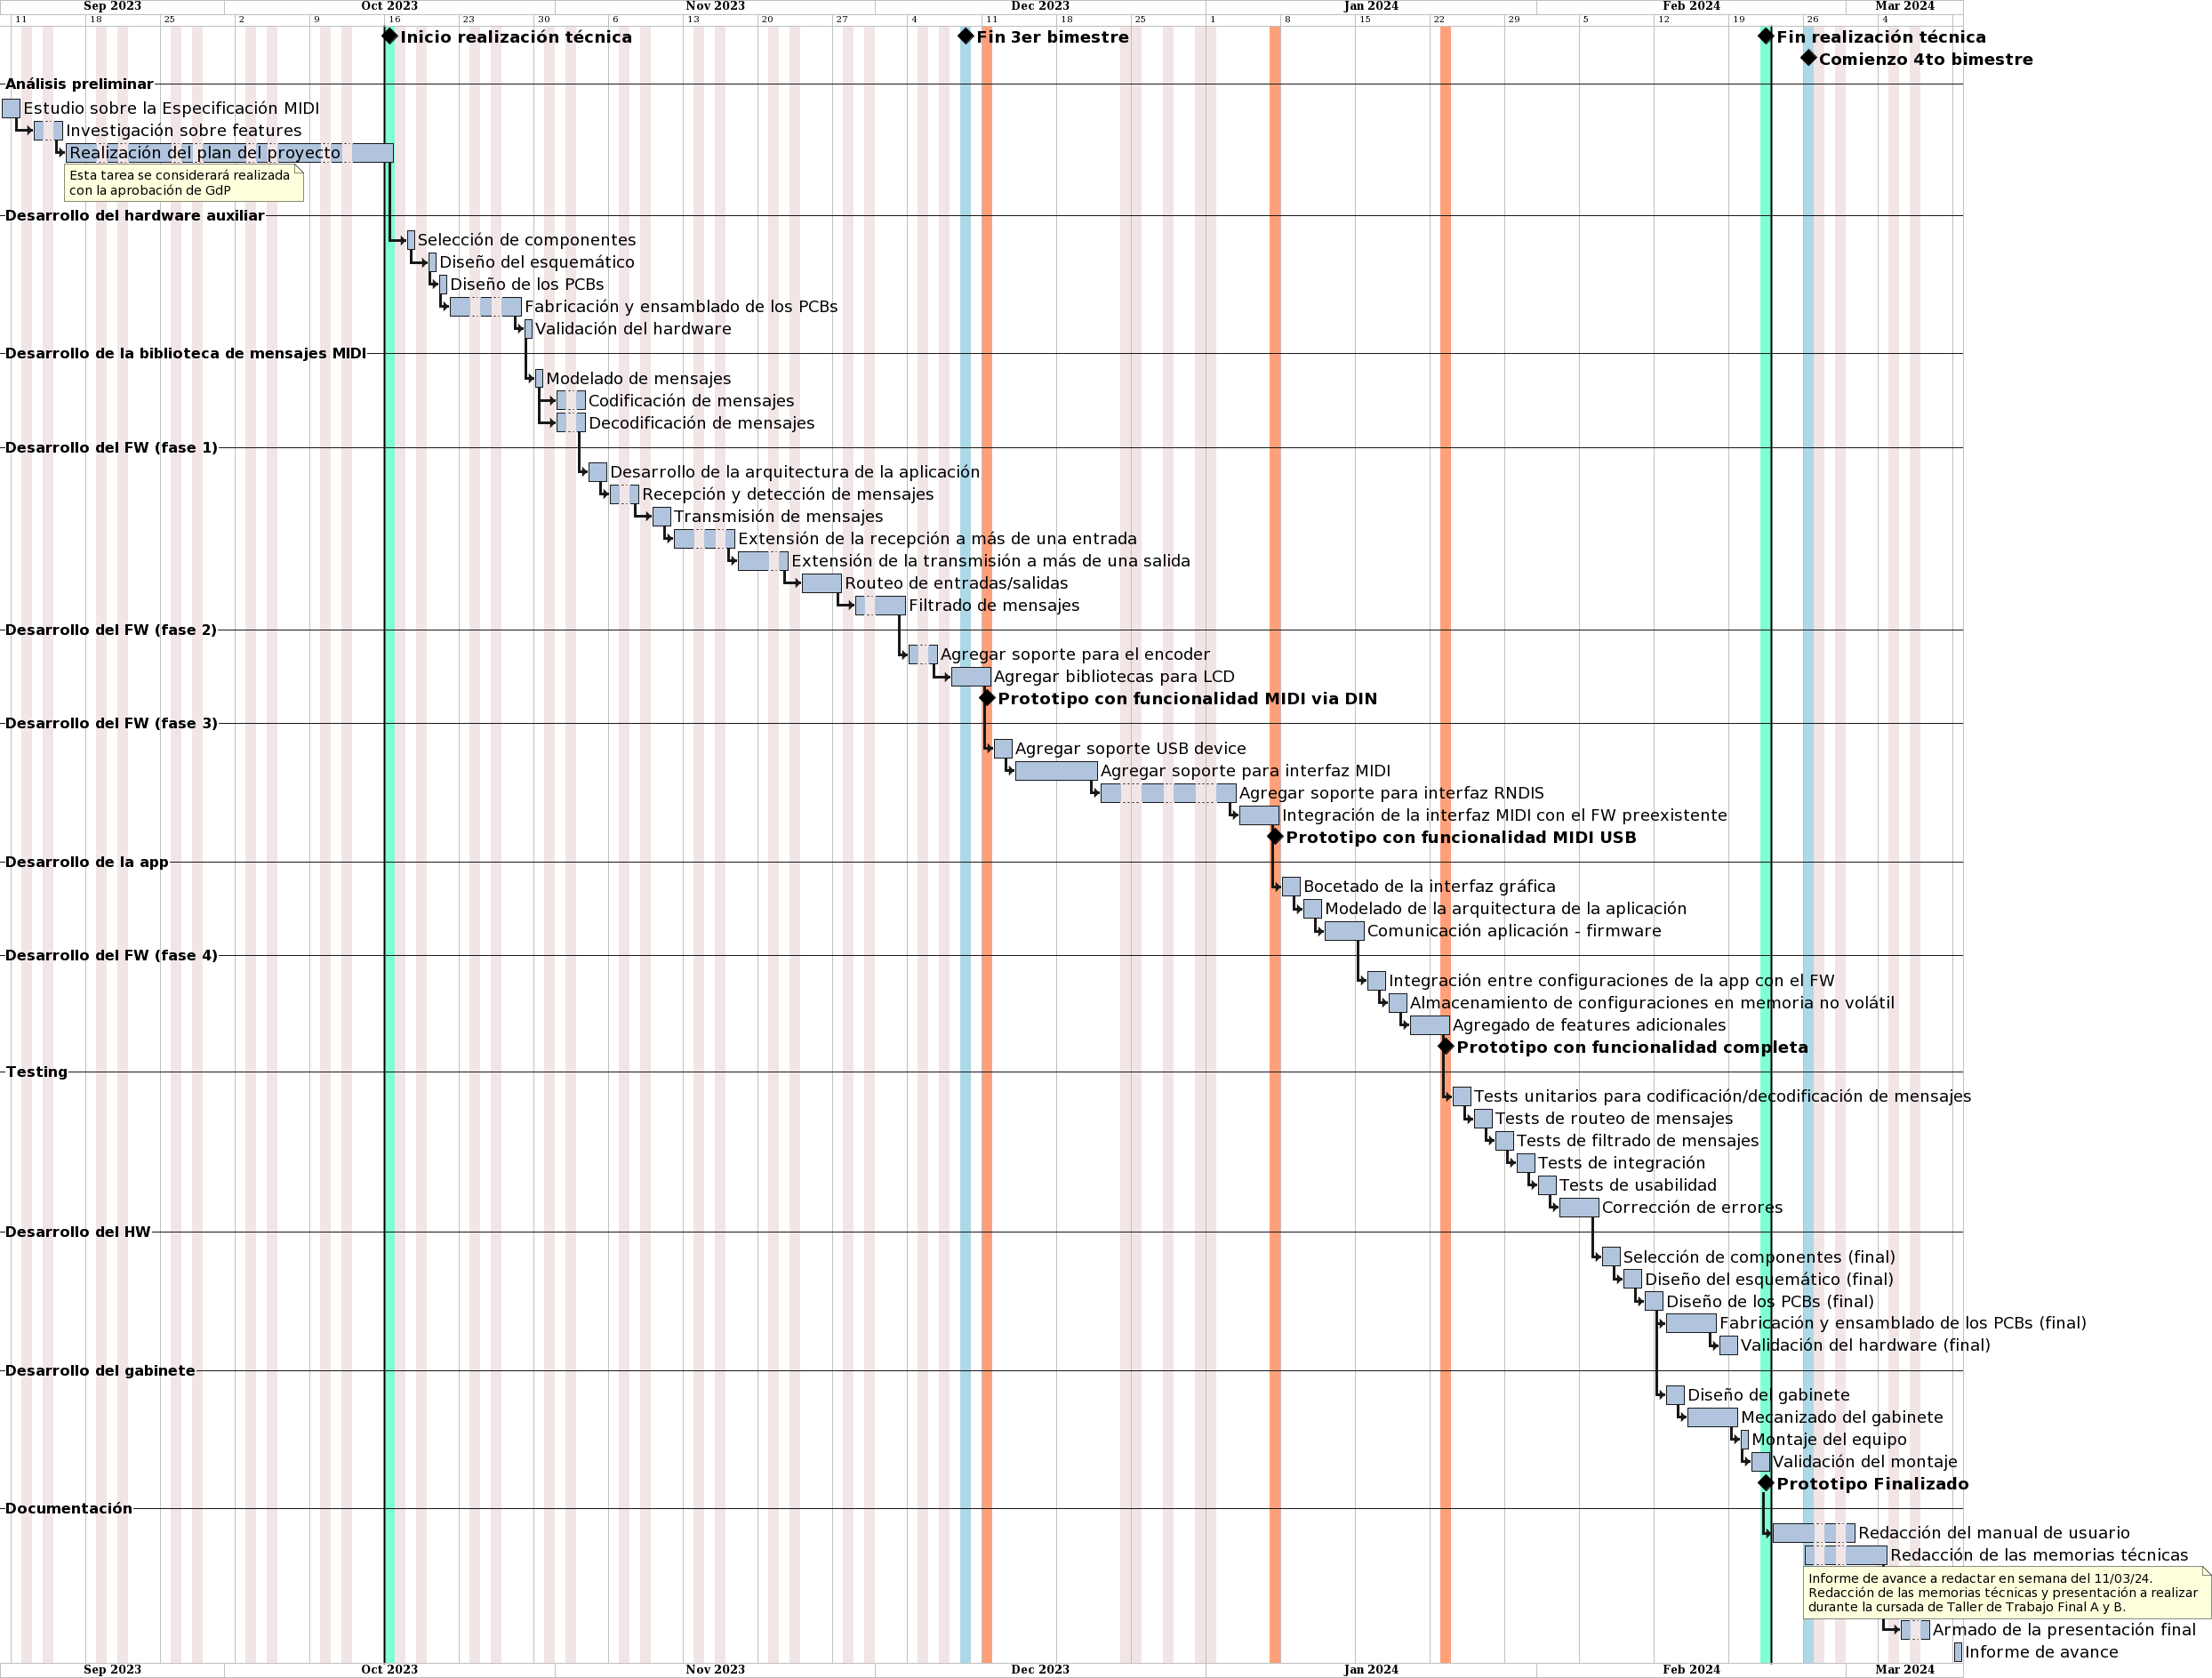
\includegraphics[height=1.05\textheight]{./Figuras/gantt.png}
		\caption{Diagrama de Gantt del proyecto.}
		\label{fig:diagGantt}
	\end{figure}
\end{landscape}

\section{12. Presupuesto detallado del proyecto}
\label{sec:presupuesto}

El presente presupuesto se encuentra en dólares estadounidenses. La conversión usada es de \$365,50 por dólar, de acuerdo con la cotización de venta del Banco Nación de la Argentina el día 25 de septiembre de 2023.

\begin{table}[htpb]
\centering
\begin{tabularx}{\linewidth}{@{}|X|c|r|r|@{}}
\hline
\rowcolor[HTML]{C0C0C0} 
\multicolumn{4}{|c|}{\cellcolor[HTML]{C0C0C0}COSTOS DIRECTOS} \\ \hline
\rowcolor[HTML]{C0C0C0} 
Descripción &
  \multicolumn{1}{c|}{\cellcolor[HTML]{C0C0C0}Cantidad} &
  \multicolumn{1}{c|}{\cellcolor[HTML]{C0C0C0}Valor unitario} &
  \multicolumn{1}{c|}{\cellcolor[HTML]{C0C0C0}Valor total} \\ \hline

Horas de Ingeniería &
  \multicolumn{1}{c|}{630} &
  \multicolumn{1}{c|}{US\$ 20} &
  \multicolumn{1}{c|}{US\$ 12600} \\ \hline

Kit de desarrollo \texttt{NUCLEO-H755ZI-Q} &
  \multicolumn{1}{c|}{1} &
  \multicolumn{1}{c|}{US\$ 30} &
  \multicolumn{1}{c|}{US\$ 30} \\ \hline

Conectores DIN-5 \texttt{KCDX-5S-S2} &
\multicolumn{1}{c|}{20} &
\multicolumn{1}{c|}{US\$ 1,58} &
\multicolumn{1}{c|}{US\$ 31,6} \\ \hline

Optoacopladores \texttt{6N137} &
\multicolumn{1}{c|}{20} &
\multicolumn{1}{c|}{US\$ 0,522} &
\multicolumn{1}{c|}{US\$ 10,44} \\ \hline

Componentes pasivos varios &
\multicolumn{1}{c|}{1} &
\multicolumn{1}{c|}{US\$ 200} &
\multicolumn{1}{c|}{US\$ 200} \\ \hline

Servicio de mecanizado de gabinetes &
\multicolumn{1}{c|}{1} &
\multicolumn{1}{c|}{US\$ 250} &
\multicolumn{1}{c|}{US\$ 250} \\ \hline

Manufactura de PCBs &
\multicolumn{1}{c|}{1} &
\multicolumn{1}{c|}{US\$ 237} &
\multicolumn{1}{c|}{US\$ 237} \\ \hline

\multicolumn{3}{|c|}{SUBTOTAL} &
\multicolumn{1}{c|}{US\$ 13359,04} \\ \hline

\rowcolor[HTML]{C0C0C0} 
\multicolumn{4}{|c|}{\cellcolor[HTML]{C0C0C0}COSTOS INDIRECTOS} \\ \hline
\rowcolor[HTML]{C0C0C0} 
Descripción &
  \multicolumn{1}{c|}{\cellcolor[HTML]{C0C0C0}Cantidad} &
  \multicolumn{1}{c|}{\cellcolor[HTML]{C0C0C0}Valor unitario} &
  \multicolumn{1}{c|}{\cellcolor[HTML]{C0C0C0}Valor total} \\ \hline

5\% de los costos directos &
\multicolumn{1}{c|}{1} &
\multicolumn{1}{c|}{US\$ 667,95} &
\multicolumn{1}{c|}{US\$ 667,95} \\ \hline

Costos de envío y logística &
\multicolumn{1}{c|}{1} &
\multicolumn{1}{c|}{US\$ 60} &
\multicolumn{1}{c|}{US\$ 60} \\ \hline

\multicolumn{3}{|c|}{SUBTOTAL} &
  \multicolumn{1}{c|}{US\$ 727,95} \\ \hline
\rowcolor[HTML]{C0C0C0}
\multicolumn{3}{|c|}{TOTAL} & \multicolumn{1}{c|}{US\$ 14086,99}
   \\ \hline
\end{tabularx}%
\end{table}


\section{13. Gestión de riesgos}
\label{sec:riesgos}

\begin{consigna}{red}
a) Identificación de los riesgos (al menos cinco) y estimación de sus consecuencias:
 
Riesgo 1: detallar el riesgo (riesgo es algo que si ocurre altera los planes previstos de forma negativa)
\begin{itemize}
	\item Severidad (S): mientras más severo, más alto es el número (usar números del 1 al 10).\\
	Justificar el motivo por el cual se asigna determinado número de severidad (S).
	\item Probabilidad de ocurrencia (O): mientras más probable, más alto es el número (usar del 1 al 10).\\
	Justificar el motivo por el cual se asigna determinado número de (O). 
\end{itemize}   

Riesgo 2:
\begin{itemize}
	\item Severidad (S): 
	\item Ocurrencia (O):
\end{itemize}

Riesgo 3:
\begin{itemize}
	\item Severidad (S): 
	\item Ocurrencia (O):
\end{itemize}


b) Tabla de gestión de riesgos:      (El RPN se calcula como RPN=SxO)

\begin{table}[htpb]
\centering
\begin{tabularx}{\linewidth}{@{}|X|c|c|c|c|c|c|@{}}
\hline
\rowcolor[HTML]{C0C0C0} 
Riesgo & S & O & RPN & S* & O* & RPN* \\ \hline
       &   &   &     &    &    &      \\ \hline
       &   &   &     &    &    &      \\ \hline
       &   &   &     &    &    &      \\ \hline
       &   &   &     &    &    &      \\ \hline
       &   &   &     &    &    &      \\ \hline
\end{tabularx}%
\end{table}

Criterio adoptado: 
Se tomarán medidas de mitigación en los riesgos cuyos números de RPN sean mayores a...

Nota: los valores marcados con (*) en la tabla corresponden luego de haber aplicado la mitigación.

c) Plan de mitigación de los riesgos que originalmente excedían el RPN máximo establecido:
 
Riesgo 1: plan de mitigación (si por el RPN fuera necesario elaborar un plan de mitigación).
  Nueva asignación de S y O, con su respectiva justificación:
  - Severidad (S): mientras más severo, más alto es el número (usar números del 1 al 10).
          Justificar el motivo por el cual se asigna determinado número de severidad (S).
  - Probabilidad de ocurrencia (O): mientras más probable, más alto es el número (usar del 1 al 10).
          Justificar el motivo por el cual se asigna determinado número de (O).

Riesgo 2: plan de mitigación (si por el RPN fuera necesario elaborar un plan de mitigación).
 
Riesgo 3: plan de mitigación (si por el RPN fuera necesario elaborar un plan de mitigación).

\end{consigna}


\section{14. Gestión de la calidad}
\label{sec:calidad}

A continuación se detallan los procedimientos de verificación y validación para los requerimientos más importantes del proyecto:

\begin{itemize} 	
	\item \textbf{Requerimiento 1.2:} \emph{El equipo deberá tener por lo menos 4 (cuatro) conectores de entrada.}
	\begin{itemize}
		\item Verificación: se elegirá esta cantidad de entradas durante la fase de diseño del firmware.
		\item Validación: se mostrará el funcionamiento del equipo con todas las entradas conectadas.
	\end{itemize}
	
	\item \textbf{Requerimiento 1.3:} \emph{El equipo deberá tener por lo menos 8 (ocho) conectores de salida.}
	\begin{itemize}
		\item Verificación: se elegirá esta cantidad de salidas durante la fase de diseño del firmware.
		\item Validación: se mostrará el funcionamiento del equipo con todas las salidas conectadas.
	\end{itemize}
	
	\item \textbf{Requerimiento 3.2:} \emph{El equipo deberá ser \emph{class-compliant} (es decir, no requerir de drivers adicionales para
	poder utilizarse desde la PC).}
	\begin{itemize}
		\item Verificación: se desarrollará el firmware de modo que se alcance este requerimiento.
		\item Validación: se mostrará la característica \emph{plug and play} del equipo o al conectarlo por el puerto USB.
	\end{itemize}
	
	\item \textbf{Requerimiento 3.4:} \emph{Los puertos MIDI de entrada y salida deberán ser accesibles desde la computadora.}
	\begin{itemize}
		\item Verificación: se desarrollará esta característica durante la fase de diseño del firmware.
		\item Validación: se mostrará el funcionamiento del equipo con esta característica.
	\end{itemize}

	\item \textbf{Requerimiento 4.1:} \emph{La comunicación Humano-Máquina más elemental se realizará mediante un display
	LCD (u OLED -a definir-) gráfico y un encoder rotativo.}
	\begin{itemize}
		\item Verificación: se analizarán distintas alternativas de pantallas y encoders de modo de elegir las opciones más adecuadas.
		\item Validación: el equipo deberá funcionar con las opciones seleccionadas.
	\end{itemize}
	
	\item \textbf{Requerimiento 4.3:} \emph{La configuración de \emph{routeo} y filtrado de mensajes se realizará a través de una aplicación gráfica.}
	\begin{itemize}
		\item Verificación: se desarrollará una aplicación con la funcionalidad requerida.
		\item Validación: se mostrará el funcionamiento del equipo con esta característica.  
	\end{itemize}
	
	\item \textbf{Requerimiento 5.2:} \emph{El equipo deberá ser capaz de almacenar al menos 16 (dieciseis) presets configurables por el usuario.}
	\begin{itemize}
		\item Verificación: se desarrollará esta característica durante la fase de diseño del firmware, y será testeada \emph{a posteriori}.
		\item Validación: se mostrará el funcionamiento del equipo con esta característica.
	\end{itemize}

	\item \textbf{Requerimiento 5.4:} \emph{La pantalla LCD deberá mostrar el preset activo.}
	\begin{itemize}
		\item Verificación: se desarrollará esta característica durante la fase de diseño del firmware, y será testeada \emph{a posteriori}.
		\item Validación: se mostrará el funcionamiento del equipo con esta característica.
	\end{itemize}

	\item \textbf{ Requerimiento 7.2:} \emph{Se deberá confeccionar un manual de uso orientado a potenciales usuarios que podrían no contar con conocimiento técnico.}
	\begin{itemize}
		\item Verificación: se incluirá la redacción del mismo en la planificación del proyecto.
		\item Validación: será parte de los entregables del proyecto.
	\end{itemize}
	
	\item \textbf{Requerimiento 8.1:} \emph{Se deberá confeccionar un manual de uso orientado a potenciales usuarios que podrían no contar con conocimiento técnico.}
	\begin{itemize}
		\item Verificación: se comprobarán los planos mecánicos del sistema.
		\item Validación: se verá la presentación del equipo.
	\end{itemize}

\end{itemize}

\section{15. Procesos de cierre}    
\label{sec:cierre}

\begin{consigna}{red}
Establecer las pautas de trabajo para realizar una reunión final de evaluación del proyecto, tal que contemple las siguientes actividades:

\begin{itemize}
	\item Pautas de trabajo que se seguirán para analizar si se respetó el Plan de Proyecto original:
	 - Indicar quién se ocupará de hacer esto y cuál será el procedimiento a aplicar. 
	\item Identificación de las técnicas y procedimientos útiles e inútiles que se emplearon, y los problemas que surgieron y cómo se solucionaron:
	 - Indicar quién se ocupará de hacer esto y cuál será el procedimiento para dejar registro.
	\item Indicar quién organizará el acto de agradecimiento a todos los interesados, y en especial al equipo de trabajo y colaboradores:
	  - Indicar esto y quién financiará los gastos correspondientes.
\end{itemize}

\end{consigna}


\end{document}
